\section{Concepts and language support}\label{sec:concepts}

We introduce two main notions: \emph{i)} individual \emph{context} and \emph{ii)
context group}, which along with a number of secondary notions form a complete
design. Context represents an environmental situation the system may find itself
in, and defines a behavioral pivot point. The software adapts to the
environmental dynamics by \emph{activating} the corresponding context. Context
groups represent collections of contexts, combine the variations of the same
functionality, and identify orthogonal aspects and mutual constraints.

\begin{figure}
\begin{center}
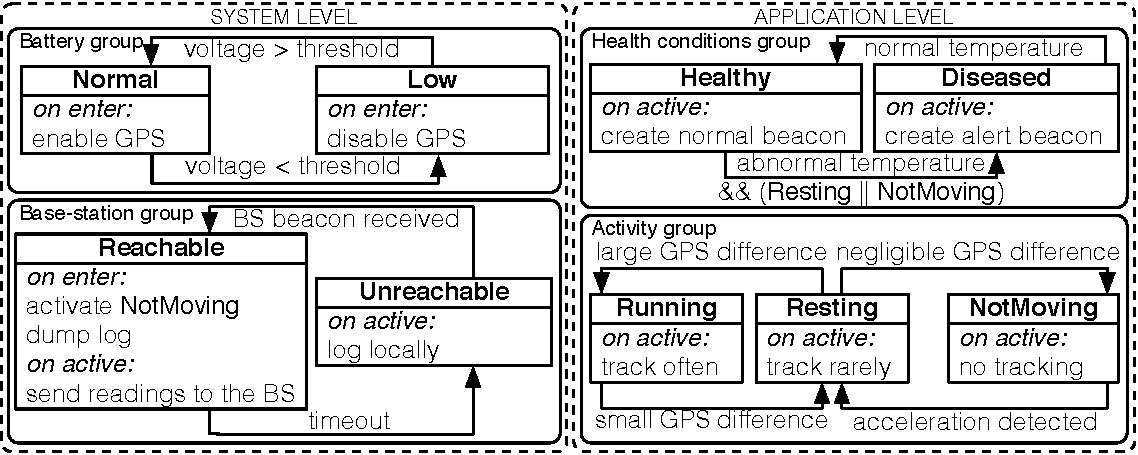
\includegraphics[scale=.45]{imgs/wildlifetracking}
\vspace{-1mm}
\caption{Wildlife monitoring application design.}
  \label{fig:design}
\vspace{-7mm}
\end{center}
\end{figure}

{\bf \conesc.} We render the concepts above in a set of COP-oriented language
constructs. Our target language nesC -- one of the most popular for programming
WSNs -- exemplifies the restrictions of CPSs such as limited memory and CPU
performance, as well as absence of memory protection. Our context-oriented
extension of nesC, called \conesc, overcomes the restrictions and brings COP to
CPSs by extending nesC modules and configurations.

\begin{figure}[!tb]
\begin{lstlisting}[style=conescframe]
context group BaseStationG {
*\lstnote{cg:layered}* layered command void report(contact_t contact);
}implementation {
*\lstnote{cg:ctx}* contexts Reachable, 
*\lstnote{cg:def}*          Unreachable is default,
*\lstnote{cg:error}*          ErrorC is error;
 // Standard nesC component wirings... }
\end{lstlisting}
\vspace{-3mm}
\caption{Context group in \conesc.}
  \label{fig:configuration}
\vspace{-7mm}
\end{figure}

The context-oriented design of an example wildlife tracking application is
displayed in Fig.~\ref{fig:design}. Context groups describe possible dynamics
corresponding to battery level, base-station availability, health conditions and
activity of an animal. In \conesc \emph{context group} extends a standard nesC
configuration and declares layered functions -- the core notion of
COP~\cite{Hirschfeld08} meant to implement a behavioral variation -- by using
the key-word \code{layered}, as shown in Fig.~\ref{fig:configuration}. Included
contexts are declared by using the key-word \code{contexts} with optional
modifiers \code{is default} to define the active context at start-up, and
optional modifier \code{is error} to specify an \emph{error} context discussed
later in this section. Explicit context activation can be initiated anywhere in
the code, as:

\vspace{-1mm}
\begin{lstlisting}[language=conesc]
activate BaseStationG.Unreachable;
\end{lstlisting}
\vspace{-1.5mm}

Contexts correspond to the separate environmental situations. For example, two
different reachability of the base-station would correspond to different
behaviors of the software. Activated context is a pivot point, where the
software changes its execution flow according to the implementation of a layered
function -- e.g. a behavioral variation. For example, in ``Reachable'' context,
as shown on line~\lstref{ct:layer} in Figure~\ref{fig:context},
function~\code{report()} sends the contacts via radio. This function represents
\emph{continuous activities}, as well as logging contacts locally as long as
``Unreachable'' context is active.

Opposite to \emph{continuous activities}, there are also \emph{one-time
operations}, such as dumping the logs on the base-station on entering the
context ``Unreachable''. In \conesc, these operations can be implemented by
using predefined events \code{activated()} and \code{deactivated()}, which are
shown on lines~\lstref{ct:activate} and~\lstref{ct:deactivate}. They are
automatically signaled when entering or leaving contexts.

The contexts transitions within the group are governed by rules. For example,
within the ``Base-station'' group, the system initiates the transition from
``Reachable'' to ``Unreachable'' whenever no beacons from the base-station are
received within a specific timeout. Contexts indicated after the key-word
\code{transitions} on line \lstref{ct:tr} represent possible outgoing
transitions. They are also possibly followed by a key-word \code{iff} to state
constraints on the transitions:

\vspace{-1mm}
\begin{lstlisting}[language=conesc]
transitions Diseased iff Resting || NotMoving;
\end{lstlisting}
\vspace{-1.5mm}

The example is in Fig.~\ref{fig:design} in the ``Health conditions'' group: when
activating the ``Diseased'' context based on body temperature, the software
should also check that either ``NotMoving'' or ``Resting'' in ``Activity group''
is currently active. Should the constraints be violated, the ``Error'' context
defined in the corresponding context group is activated. Indeed, a diseased
animal is probably not very active. Otherwise, developers might have not
correctly caught the contexts' evolution.

The required adaptation may affect several context groups. For example, whenever
the base-station is ``Reachable'', context ``NotMoving'' should also be activated.
The latter saves energy by disabling the GPS-sensor, since the base-station is
static and deployed in a known location. To this end, the keyword
\code{triggers} on line~\lstref{ct:trigger} binds the activation across the
groups. For example, the context ``NotMoving'' is activated on entering the
``Reachable'' context, as specified in Figure~\ref{fig:design}.


\begin{figure}[!tb]
\begin{lstlisting}[style=conescframe]
context Reachable {
*\lstnote{ct:tr}* transitions Unreachable;
*\lstnote{ct:trigger}* triggers NotMoving;
 uses interface Radio;
} implementation {
*\lstnote{ct:layer}* layered command void report(contact_t contact){
  call Radio.send(contact);}
*\lstnote{ct:activate}* event void activated(){// Dump logs on base-station }
*\lstnote{ct:deactivate}* event void deactivated(){ // Radio clean-up }}
\end{lstlisting}
\vspace{-3mm}
\caption{Individual context in \conesc.}
  \label{fig:context}
\vspace{-7mm}
\end{figure}
